\section{Results}\label{sec:results}

Table~\ref{tab:scorecard} gives the answer first. The QDG does what Section~\ref{sec:core} predicts on every pair the
oracle can check, comes within a few points of the smallest complete slice, holds under noise, and costs milliseconds.
It is not guaranteed to contain a fault, since a fault can delete the very interaction a slice would follow, and RQ3
measures how often that happens. The subsections answer each question for every rule.

\begin{table}[t]
  \centering
  \caption{The QDG on every question of the study}
  \label{tab:scorecard}
  \footnotesize\setlength{\tabcolsep}{3pt}\renewcommand{\arraystretch}{1.12}
  \newcommand{\sep}{\arrayrulecolor{black!25}\hline\arrayrulecolor{black}}
  \begin{tabular}{@{}l >{\raggedright\arraybackslash}p{2.0cm} >{\raggedright\arraybackslash}p{4.15cm}@{}}
    \toprule
    \textbf{Question} & \textbf{Expected} & \textbf{Observed} \\
    \midrule
    Sound (RQ1) & every input, Theorem~\ref{thm:sound} & \numRqOneLcUnsound{} wrong slices of \numNPairs{} pairs, and of \numCorpusLSoundPairs{} on corpus~L \\ \sep
    Complete (RQ1) & Proposition~\ref{prop:complete} & recall \numRqOneLcRecall{} of the measured dependences \\ \sep
    Size (RQ1) & not minimal & \numLcExcess{} points above the dependence set, equal to it on \numLcExact{} pairs \\ \sep
    Noise (RQ2) & local noise, Theorem~\ref{thm:sound} & trace distance at most \numNoiseLcCrossExactMax{} \\ \sep
    Faults (RQ3) & no guarantee & contains \numRqThreeContainLc{} of the faults, \numSizeCtlLcGain{} points above a random set of its size \\ \sep
    Cost (RQ4) & one pass & at most \numCostLcMaxCritMs{}~ms per criterion \\
    \bottomrule
  \end{tabular}
\end{table}

\subsection{RQ1: Which rules give sound and complete slices?}

\begin{table}[t]
  \centering
  \caption{Slices of the \numNPairs{} corpus-A pairs for RQ1}
  \label{tab:rq1}
  \footnotesize\setlength{\tabcolsep}{3pt}\renewcommand{\arraystretch}{1.12}
  \newcommand{\sep}{\arrayrulecolor{black!25}\hline\arrayrulecolor{black}}
  \begin{tabular}{@{}l r r r r r@{}}
    \toprule
    \textbf{Rule} & \textbf{Wrong} & \textbf{Dynamic} & \textbf{Recall} & \textbf{Precision} & \textbf{Size} \\
    \midrule
    Dependence set$^{a}$ & -- & -- & 1.000 & 1.000 & \numDepFloor{} \\
    \midrule
    \rowcolor{blue!7}\textbf{QDG} & \textbf{\numRqOneLcUnsound{}} & \numLcDynamicUnsound{} & \textbf{\numRqOneLcRecall{}} & \numRqOneLcPrecision{} & \numRqOneLcSize{} \\ \sep
    Def-use & \numRqOneDuUnsound{} & \numDuDynamicUnsound{} & \numRqOneDuRecall{} & \numRqOneDuPrecision{} & \numRqOneDuSize{} \\ \sep
    Classical PDG & \numCpdgUnsound{} & \numCpdgDynamicUnsound{} & \numCpdgRecall{} & \numCpdgPrecision{} & \numCpdgSize{} \\ \sep
    QPDG~\cite{yu2025qpdg} & \numRqOneYzUnsound{} & \numYzDynamicUnsound{} & \numRqOneYzRecall{} & \numRqOneYzPrecision{} & \numRqOneYzSize{} \\ \sep
    QPDG, flow-sensitive$^{b}$ & \numYzfUnsound{} & \numYzfDynamicUnsound{} & \numYzfRecall{} & \numYzfPrecision{} & \numYzfSize{} \\
    \midrule
    Commutation$^{c}$ & \numLcqUnsound{} & \numLcqDynamicUnsound{} & \numLcqRecall{} & \numLcqPrecision{} & \numLcqSize{} \\ \sep
    Commutation, symbolic$^{c}$ & \numLcqsUnsound{} & \numLcqsDynamicUnsound{} & \numLcqsRecall{} & \numLcqsPrecision{} & \numLcqsSize{} \\ \sep
    State-based & \numRqOneQUnsound{} & \numQDynamicUnsound{} & \numRqOneQRecall{} & \numRqOneQPrecision{} & \numRqOneQSize{} \\
    \bottomrule
  \end{tabular}\\[3pt]
  \begin{minipage}{\columnwidth}\footnotesize
  Wrong counts the slices that do not preserve the criterion at $\ket{0\dots0}$, a lower bound for every rule but the
  QDG, which is sound for all inputs, and Dynamic those among the \numNDynamicPairs{} pairs in dynamic circuits.
  Recall and precision are against the dependence set, and size is the mean share of the circuit. $^{a}$\,The
  smallest slice that contains every dependence, a reference and not a rule. $^{b}$\,Exploratory, the variant of
  Section~\ref{sec:rules}. $^{c}$\,On the \numLcqApplicable{} pairs where Qiskit's pass
  applies, \numLcqDynamicN{} of them dynamic.
  \end{minipage}
\end{table}

One choice decides soundness, what a controlled gate writes. The classical PDG, which lets a CNOT write only its
target, misses \numCpdgMissTotal{} dependences over the \numNPairs{} pairs, and all but \numCpdgMissFeedback{} of
them, \numCpdgMissControlPct{}, follow from reading a control as unchanged. Of the misses, \numCpdgMissSameWire{} are
controlled gates whose control is the criterion qubit, \numCpdgMissKickback{} reach the criterion only through such
a gate, \numCpdgMissWritten{} reach it through a control further along the chain, and only \numCpdgMissFeedback{}
pass through classical feedback. As a result, Table~\ref{tab:rq1} shows, the classical PDG gives a wrong slice for
\numCpdgUnsound{} of the pairs, or \numCpdgUnsoundPct{}, with a 95\% interval of \numCcCpdgUnsound{} when the
\numCcFamilies{} algorithm families are resampled as clusters. Its control dependence matters only on dynamic
circuits, where it is wrong on \numCpdgDynamicUnsound{} pair against \numDuDynamicUnsound{} for def-use.

Many of these wrong slices look right. Of the \numCpdgUnsound{}, \numFdCpdgZMatch{}, or \numFdCpdgZMatchPct{}, give
the criterion the same distribution of outcomes in the computational basis as the whole circuit, so only
\numFdCpdgObservable{} pairs, \numFdCpdgObservablePct{} of all, are wrong in what a terminal measurement reads. The
others are wrong in phase, which a histogram check accepts but which changes the outcome once the slice is composed
with later gates or measured in another basis. Testing meets the same limit, since phase-flip faults escape
measurement in the computational basis~\cite{oldfield2024faster}. A developer who checks a slice by its outcomes
would therefore accept almost half of the wrong ones. As H1 expects by construction, state-based pruning, which
starts from the QDG slice, is wrong on fewer pairs than def-use, \numRqOneQUnsound{} against \numRqOneDuUnsound{}
(exact McNemar, Holm \numHOnePHolm{}).

The QDG is sound on every pair and recovers every measured dependence, as Theorem~\ref{thm:sound} and
Proposition~\ref{prop:complete} predict. The QPDG is sound too, since its slices contain the QDG's, but its
entanglement edges add only operations that are not dependences, and its slices grow from \numRqOneLcSize{} to
\numRqOneYzSize{} of the circuit. The flow-sensitive variant still keeps \numYzfExcess{} points above the dependence
set, and a graph with one entanglement edge per two-qubit gate gives exactly the QDG slice on all
\numFdFourEdgeNoClosureEqual{} pairs it applies to, so the excess comes from closing these edges transitively. Under the
reading in which a controlled gate writes only its targets, the QPDG is wrong on \numYzRoUnsound{} pairs. On the
\numCorpusLSoundPairs{} pairs of corpus~L that the oracle can check exactly, the QDG and the QPDG are sound everywhere,
while def-use is wrong on \numCorpusLWrongDu{}.

\begin{figure}[t]
  \centering
  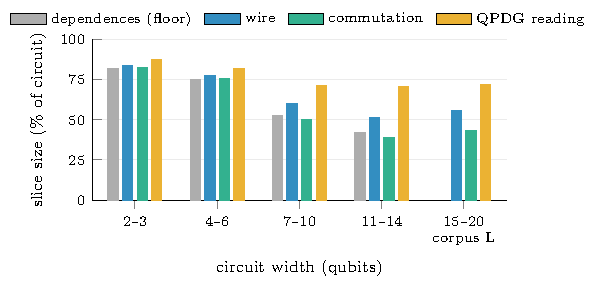
\includegraphics[width=\columnwidth]{figures/fig_size.pdf}
  \caption{Mean slice size by circuit width, for RQ1. The dependence set is the floor that every complete slice
  contains. Corpus~L has no dependence set, since measuring one there would need more simulation than the oracle can
  do exactly.}
  \label{fig:size}
\end{figure}

The rules nest, and Fig.~\ref{fig:size} shows how far apart they are. On all \numNestPairs{} pairs the dependence set
lies within the QDG slice and the QDG slice within the QPDG slice. Restricted to its dependence set, every circuit
preserves the criterion at $\ket{0\dots0}$, so at that input the dependence set is itself a correct slice, the
smallest one that contains every dependence. It makes up \numDepFloor{} of a circuit on average. The QDG slice keeps only
\numLcExcess{} percentage points more and equals it on \numLcExact{} of the \numNPairs{} pairs, while the QPDG keeps
\numYzExcess{} points more, \numYzLcExcessRatio{} times as much code that cannot change the criterion. The gap grows
with width. At \numWElevenLo{} to \numWElevenHi{} qubits the QDG slice keeps \numWElevenLc{} of the circuit and on
corpus~L \numCorpusLSizeLc{}, while the QPDG stays near \numCorpusLSizeYz{}, because it links the operations of a whole
coupling component. Commutation pruning falls below the dependence set, to \numWElevenLcq{} at the same widths,
because it is sound for fixed angles but not complete. It can drop an operation where a fault would change the
criterion, as the identity gate of line~38 in Fig.~\ref{fig:bv} shows, which is why completeness, not size, is what a
developer needs from a slice.

\subsection{RQ2: How much precision beyond the QDG slice is safe?}

\begin{figure}[t]
  \centering
  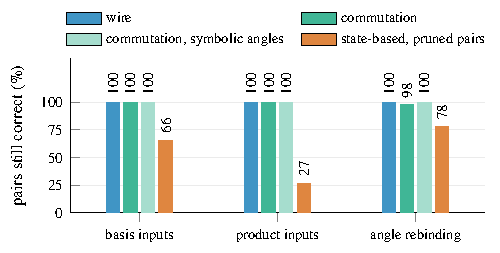
\includegraphics[width=\columnwidth]{figures/fig_robust.pdf}
  \caption{Share of pairs whose slice, computed at $\ket{0\dots0}$, stays correct in all \numRobDraws{} draws of each
  input regime, for RQ2. Commutation is shown on the \numLcqApplicable{} pairs where Qiskit's pass applies,
  state-based pruning on the \numHThreePrunedN{} pairs it prunes, and angle rebinding on the pairs of circuits with
  rotation angles.}
  \label{fig:robust}
\end{figure}

Both refinements make slices smaller, but only commutation pruning keeps them correct for fixed angles. State-based
pruning shrinks the QDG slice by \numHTwoDiff{} percentage points of the circuit (95\% CI \numHTwoCILow{} to
\numHTwoCIHigh{}) and is smaller on \numHTwoSmaller{} pairs (H2, Wilcoxon, Holm \numHTwoPHolm{}).
Fig.~\ref{fig:robust} shows what that costs. Of the pairs it prunes, the slice stays correct for all random product
inputs on only \numHThreePrunedRate{}, and over all pairs on \numHThreeRate{} (Wilson CI \numHThreeCILow{} to
\numHThreeCIHigh{}, \numCcHThree{} with families as clusters), far below the pre-registered threshold of 95\%, so H3
fails. A state-based slice is a property of one input, not of the program.

Commutation pruning is smaller than the QDG slice on \numLcqSmallerThanLc{} of \numLcqApplicable{} pairs, stays
correct on every random basis and product input, and fails only when the angles change, on \numRobLcqParamFail{} of
\numRobLcqParamN{} pairs of variational circuits. Its symbolic variant, at a mean size of \numLcqsSize{} against
\numLcqSize{}, stays correct on every pair in every regime. Its recall of \numLcqRecall{} shows that it misses
dependences, since a different gate in place of one it drops could change the criterion.

Under depolarizing noise at two-qubit error rates of $10^{-3}$ to $3\cdot10^{-2}$, a pre-registered descriptive
analysis, the criterion's states under the QDG slice and the whole circuit differ by a trace distance of at most
\numNoiseLcCrossExactMax{} where the simulation is exact, rounding error as Theorem~\ref{thm:sound} predicts, while the
state-based slice differs in \numNoiseQCrossExactNonzero{} of \numNoiseQCrossExactN{} exact runs, by up to
\numNoiseQCrossExactMax{}, because it removes noisy gates that the program executes~\cite{preskill2018nisq}.

\subsection{RQ3: What does each rule do to fault localization?}

\begin{table}[t]
  \centering
  \caption{Faults and slices on the \numRqThreeUnits{} seeded-fault units, for RQ3}
  \label{tab:rq3}
  \footnotesize\setlength{\tabcolsep}{3pt}\renewcommand{\arraystretch}{1.12}
  \newcommand{\sep}{\arrayrulecolor{black!25}\hline\arrayrulecolor{black}}
  \begin{tabular}{@{}l r r r r r@{}}
    \toprule
    \textbf{Slice} & \textbf{Contains} & \textbf{Size} & \textbf{Random} & \textbf{Gain} & \textbf{EXAM} \\
    \midrule
    Whole circuit & 100\% & 100\% & -- & -- & \numMbflAllExamAll{} \\
    \midrule
    \rowcolor{blue!7}\textbf{QDG} & \numRqThreeContainLc{} & \numRqThreeSizeLc{} & \numSizeCtlLcRandom{} & \numSizeCtlLcGain{} & \numMbflAllExamLc{} \\ \sep
    QPDG & \numRqThreeContainYz{} & \numRqThreeSizeYz{} & \numSizeCtlYzRandom{} & \numSizeCtlYzGain{} & \numMbflAllExamYz{} \\ \sep
    Classical PDG & \numRqThreeContainCpdg{} & \numRqThreeSizeCpdg{} & \numSizeCtlCpdgRandom{} & \numSizeCtlCpdgGain{} & \numMbflAllExamCpdg{} \\ \sep
    Def-use & \numRqThreeContainDu{} & \numRqThreeSizeDu{} & \numSizeCtlDuRandom{} & \numSizeCtlDuGain{} & \numMbflAllExamDu{} \\ \sep
    State-based & \numRqThreeContainQ{} & \numRqThreeSizeQ{} & \numSizeCtlQRandom{} & \numSizeCtlQGain{} & \numMbflAllExamQ{} \\
    \bottomrule
  \end{tabular}\\[3pt]
  \begin{minipage}{\columnwidth}\footnotesize
  Contains is the share of units whose slice of the faulty circuit contains the fault site, size the mean share of the
  circuit, Random the containment of a random set of the slice's size, and Gain the difference in percentage points.
  EXAM is the mean score of mutation-based fault localization of Section~\ref{sec:design}, lower being better, on
  the \numMbflAllN{} sampled units whose fault every slice contains.
  \end{minipage}
\end{table}

Table~\ref{tab:rq3} shows that a slice that contains the fault more often is also larger, so containment has to be
read against a random set of the slice's size. The QDG slice contains the fault in \numRqThreeContainLc{} of the units
and the QPDG slice in \numRqThreeContainYz{}, but a random set of the QPDG's size already contains it in
\numSizeCtlYzRandom{}, so per unit of size the QDG locates faults better, \numSizeCtlLcGain{} points above random
against \numSizeCtlYzGain{} for the QPDG. Against
a random set of its own size, every rule contains the fault more often, the QDG by \numSizeCtlLcGain{} points (family CI
\numSizeCtlLcGainCi{}), so containment is not only a matter of size. All \numLcMissTotal{} units whose fault the QDG
slice misses are omission faults, a removed control (\numLcMissCrm{}), a re-targeted operand (\numLcMissQsw{}), a
removed preparation of an entangling gate (\numLcMissEnt{}) or a deleted gate (\numLcMissDel{}). Each deletes the
interaction that the slice of the faulty program would follow, so the place of the missing operation is not in the
slice. The QPDG contains \numLcMissYzContained{} of them only because its closure still links operations that the faulty
program no longer connects.

State-based pruning lowers containment by \numHFourDiffAbs{} percentage points against the QDG slice (95\% CI
\numHFourCILow{} to \numHFourCIHigh{}, \numCcHFour{} with families as clusters), so H4, which allowed a loss of at most
five points, fails. In \numCQFour{} units the QDG slice contains the fault and the state-based slice does not. Pruning
removes an operation when the criterion is uncorrelated with its qubits at the input, so a fault that breaks a
correlation can make the faulty operation look irrelevant to the single criterion qubit, and a joint criterion over all
wrong qubits recovers \numCQFourRecovered{} of these units. Where both slices contain the fault, the state-based slice
is smaller by \numHFiveSizeDiff{} operations on average, so H5 holds, but its EXAM score is higher by
\numHFiveExamQHigher{}.

Slices do not improve mutation-based fault localization. On the \numMbflAllN{} units whose fault every slice contains,
ranking within any slice reaches the fault after \numMbflAllExaminedMin{} to \numMbflAllExaminedMax{} operations on
average, as ranking over the whole circuit does, and since EXAM divides by the number of operations ranked, the whole
circuit scores lowest.

On the \numLinesUnits{} real Bugs4Q units whose faulty lines map to the program, the QDG line slices keep every faulty
line and \numLinesLcMean{} of \numLinesFullMean{} lines on average, so on these small programs slicing barely reduces
what there is to read. Def-use, which equals the classical PDG on these unitary programs, loses the faulty line in
\numLinesDuMissed{} of the units.

\paragraph*{Language models}
Asked to list the operations that can affect a qubit, Claude Sonnet~5.5 and Haiku~5.5 recall \numTOneSonnetRecall{}
and \numTOneHaikuRecall{} of the dependences and both Qwen models \numTOneQwenMidRecall{}, where the QDG slice recalls
them all, and Sonnet recalls only \numTOneSonnetKick{} of those through kickback. Asked to name the faulty operation,
no model does better with any slice than with the whole circuit by more than a fraction of a point, and Sonnet has
the fault in its top three for \numTTwoSonnetQ{} of the units with the state-based slice, \numTTwoSonnetQVsLcLoss{}
points below the QDG slice (95\% CI \numTTwoSonnetQVsLcCI{}, exact McNemar \numTTwoSonnetQVsLcP{}). A model thus misses
dependences that a slicer finds by rule, yet a slice does not help it localize a fault, and a pruned slice hurts it.

\subsection{RQ4: What does it cost?}

The QDG slice costs at most \numCostLcMaxCritMs{}~ms per criterion at every depth.
State-based pruning, which simulates the circuit for every candidate removal, exceeds the limit of \numCostWallLimit{}~s
for \numCostDepthEightyOverLimit{} of the \numCostDepthCircuits{} circuits at the second-largest depth and for all
\numCostDepthOneSixtyOverLimit{} at the largest, grows exponentially with width, and completes on
\numCorpusLCompleted{} of the \numCorpusLCircuits{} circuits of corpus~L. Building the QPDG takes
\numCostBuildDepthForty{}~s at depth \numCostMeasuredDepthForty{} and \numCostBuildDepthOneSixty{}~s at depth
\numCostMeasuredDepthOneSixty{} in the median, against milliseconds for the QDG slice, because its closure links every
pair of operations on a coupling component while the QDG needs only the operations on each qubit.
